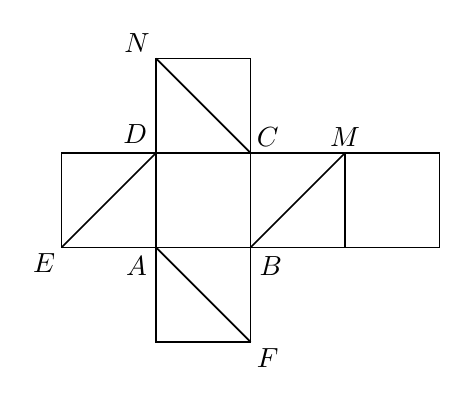
\begin{tikzpicture}[x=1cm,y=1cm,line width=.6pt,font=\normalsize]
% cube net, side 1.2
\coordinate (A) at (0,0);
\coordinate (B) at (1.2,0);
\coordinate (C) at (1.2,1.2);
\coordinate (D) at (0,1.2);
\coordinate (N) at (0,2.4);
\coordinate (Ct) at (1.2,2.4);
\coordinate (E) at (-1.2,0);
\coordinate (El) at (-1.2,1.2);
\coordinate (F) at (1.2,-1.2);
\coordinate (Fb) at (0,-1.2);
\coordinate (M) at (2.4,1.2);
\coordinate (Mb) at (2.4,0);
\coordinate (R1) at (3.6,0);
\coordinate (R2) at (3.6,1.2);
% center square
\draw (A)--(B)--(C)--(D)--cycle;
% top square
\draw (D)--(N)--(Ct)--(C)--cycle;
\draw (N)--(C);
% left square
\draw (E)--(A)--(D)--(El)--cycle;
\draw (E)--(D);
% bottom square
\draw (A)--(B)--(F)--(Fb)--cycle;
\draw (A)--(F);
% right squares
\draw (B)--(C)--(M)--(Mb)--cycle;
\draw (R1)--(R2)--(M)--(Mb)--cycle;
\draw (B)--(M);
\node[above left,inner sep=2pt] at (N) {$N$};
\node[above left,inner sep=3pt] at (D) {$D$};
\node[above right,inner sep=2pt] at (C) {$C$};
\node[above,inner sep=2pt] at (M) {$M$};
\node[below left,inner sep=2pt] at (E) {$E$};
\node[below left,inner sep=3pt] at (A) {$A$};
\node[below right,inner sep=3pt] at (B) {$B$};
\node[below right,inner sep=2pt] at (F) {$F$};
\end{tikzpicture}
